\documentclass{beamer}

%%%%% Definition du theme de la présentation
%% Theme 1 'Warsaw'
%\usepackage{beamerthemeWarsaw}

%% Theme 2 'PaloAlto'
\usetheme{PaloAlto}
\useoutertheme{sidebar}
\useinnertheme[shadow=true]{rounded}
\usecolortheme{orchid}
\usecolortheme{whale}
\setbeamercolor*{frametitle}{parent=palette primary}
\setbeamerfont{block title}{size={}}


\usepackage[frenchb]{babel}
\usepackage[utf8x]{inputenc}
\usepackage{graphicx}

\author[Fontorbe, Guillaume, Monediere, Rubagotti]{Fontorbe Jordan, Guillaume Arthur, Monediere Tristan, Rubagotti Joris}
\title{Android au pays des liseuses}
\subtitle{Proposé et encadré par : Ollinger Nicolas}
\institute{Université d'Orléans}
\date{23 Mai 2013}
\logo{
\includegraphics[height=1cm]{univorleans}}

% Suppression de la barre de navigation
\beamertemplatenavigationsymbolsempty

%% Macro permettant d'afficher le plan de chaque section au début de celle-ci
\AtBeginSection[]{
   \begin{frame}
%   \begin{center}{\Large Plan }\end{center}
\begin{small}
   \tableofcontents[currentsection,hideothersubsections]
\end{small}
   \end{frame} 
}

\begin{document}

\maketitle
\tableofcontents[hideallsubsections]

%%% Plan :
%Intro
%Description générale du logiciel
%Architecture
%point technique
%exemple de fonctionnement
%la suite

\section[Intruduction]{Introduction au domaine}


\subsection[E-Ink]{Technologie E-Ink}
\begin{frame}{Technologie E-Ink}
	%% A compléter par Arthur
\end{frame}


\subsection[Sony PRS-T1]{Liseuse Sony PRS-T1}

\begin{frame}{Caractéristiques principales} %% Liseuse en générale
	\begin{block}{Caractéristiques Sony PRS-T1}
		\begin{itemize}
			\item Processeur iMX508
			\item Écran E-Ink 6 pouces
			\item Résolution jusqu'à 16 niveaux de gris
			\item Interfaces USB
			\item WiFi
			\item Mémoire : 2Go (extensible par microSD)
		\end{itemize}
	\end{block}
\end{frame}

\begin{frame}{Processeur iMX508} %% partie iMX508
	\begin{block}{iMX508}
	\begin{itemize}
		\item{Développé par Freescale}
		\item{Architecture ARM Cortex A8}
		\item{Faible consommation d'énergie}
		\item{Bonnes performances}
		\item{Contrôleur d'écran intégré}
	\end{itemize}
	\end{block}
\end{frame}

\begin{frame}{Modules}
	\begin{block}{EPDC (Electrophoretic Display Controller)}
		\begin{itemize}
			\item{Dirige les signaux (waveform)}
			\item{Mise à jour partielle ou totale}
		\end{itemize}
	\end{block}
	\begin{block}{ePXP (enhanced Pixel Pipeline}
		\begin{itemize}
			\item Transparence
			\item Rotation d'image
			\item Agrandissement / Réduction d'image
		\end{itemize}
	\end{block}
\end{frame}

\begin{frame}{Architecture du processeur iMX508} %% Schéma
	\begin{figure}
		\begin{center}
			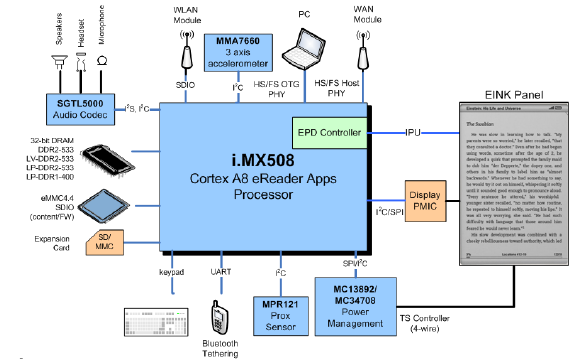
\includegraphics[scale=0.65]{iMX508.png}
		\end{center}
	\end{figure}
\end{frame}

\begin{frame}{Hack de la liseuse}
	\begin{block}{Mise à jour du firmware}
		\begin{itemize}
			\item Nécessite les clés privés de Sony
			\item Accès total à la liseuse
			\item Risque d'endommager la liseuse
		\end{itemize}
	\end{block}
	\begin{block}{Mode Recovery}
		\begin{itemize}
			\item Nécessite la recompilation du noyau
			\item Modifications sans risques
		\end{itemize}
	\end{block}
\end{frame}

\section[Description]{Description générale du logiciel}
\subsection[Objectifs]{Les attentes définies au début du projet}
\begin{frame}
\begin{enumerate}
\item
{
\begin{itemize}
\item{Lecture de la documentation}
\item{Compréhension des différentes couches matérielles et logicielles}
\item{Production d'un document de synthèse (\textbf{Mémoire intermédiaire})}
\end{itemize}
}
\item
{
\begin{itemize}
\item{Ajout du gadget USB au noyau}
\item{Connexion via SSH}
\item{Ajout du support E-ink à DirectFB}
\end{itemize}
}
\end{enumerate}
\end{frame}
\section{Architecture}
\subsection{Le système de fichiers}
\begin{frame}
\frametitle{Le système de fichiers}

\begin{block}{Image initial}
\begin{itemize}
\item Busybox
\item Un serveur DHCP
\item Un deamon telnet
\item Un accès au port USB en mode série 
\end{itemize}
\end{block}

\begin{block}{Image final}
\begin{itemize}
\item Un accès au port USB par connexion Ethernet
\item Le support du protocole SSH
\item La librairie DirectFB
\end{itemize}
\end{block}

\end{frame}

\subsection{Driver, ioctl et DirectFB}

\begin{frame}
\frametitle{Driver et ioctl}

\begin{block}{Définition ioctl}
\begin{itemize}
\item Appel système pour des opérations d'entrée/sortie
\item Prend en paramètre un code requête
\end{itemize}
\end{block}
\begin{block}{Les fonctions ioctl du driver permettent :}
\begin{itemize}
\item Mettre à jour l'affichage de l'écran
\item Récupérer des informations relatifs au driver (température, waveform, ...)
\item Modifier des paramètres du driver (température, waveform, ...)
\end{itemize}
\end{block}

\end{frame}

\begin{frame}
\frametitle{DirectFB}

\begin{block}{Intérêts}
\begin{itemize}
\item Ensemble d'API graphiques
\item Interaction directe avec le framebuffer 
\item Aucune modification du kernel
\item Aucune dépendance (sauf libc mais déjà présent)
\end{itemize}
\end{block}

\end{frame}

\begin{frame}
\frametitle{Schéma fonctionnement DirectFB}

\begin{center}
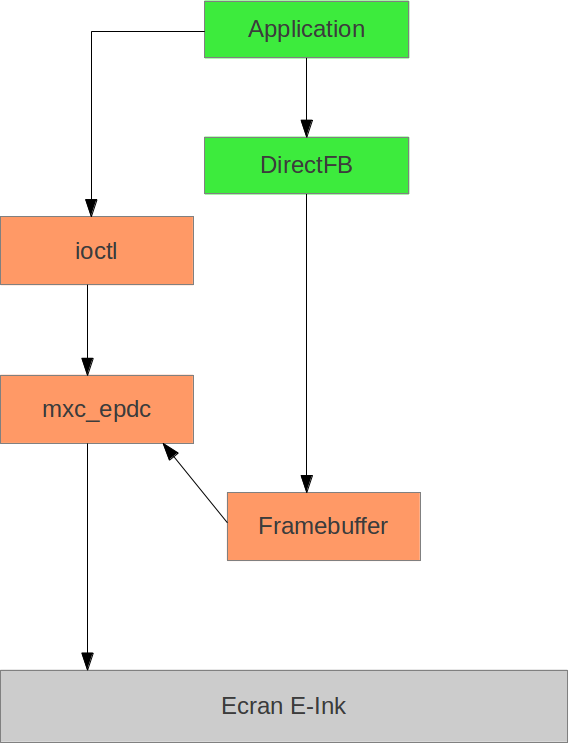
\includegraphics[scale=0.3]{schema_direct_fb.png}
\end{center}

\end{frame}


\section{Points techniques}

\subsection{La cross-compilation}
\begin{frame}{La cross-compilation}
\begin{block}{Multiple plateformes}
\begin{itemize}
\item Développement sur plusieurs systèmes d'exploitation
\item Choix du compilateur difficile
\end{itemize}
\end{block}

\begin{block}{Scratchbox}
\begin{itemize}
\item Environnement de cross-compilation
\item Machine virtuelle reproduisant une plate-forme ARM 
\item Simplification des commandes de compilation
\end{itemize}
\end{block}
\end{frame}

%	- DirectFB et ioctl
%		- ioctl
%			- les différentes commandes ioctls
%				- SEND_UPDATE
%					- struture mxcfb_update_data 
%					- diffrents champs
%				- MXCFB_WAIT_FOR_UPDATE_COMPLETE
%				- différentes ioctls

\subsection{Le driver et les ioctl}
\begin{frame}[fragile]{Les ioctl}
	\begin{block}{Les commandes ioctl}
		\begin{itemize}
			\item MXCFB\_SEND\_UPDATE 
				\begin{itemize}
					\item la structure mxcfb\_update\_data 
							\begin{itemize}
								\item update\_region
								\item waveform\_mode
								\item update\_mode
								\item update\_marker
								\item temp
								\item flags
								\item alt\_buffer\_data
							\end{itemize}
				\end{itemize}
		\end{itemize}
	\end{block}
\end{frame}

\begin{frame}{Les ioctl}
	\begin{block} {Les commandes ioctl}
		\begin{itemize}
				\item MXCFB\_WAIT\_FOR\_UPDATE\_COMPLETE
			\begin{itemize}
				\item synchronisation de la mise à jour définie par l'update marker
			\end{itemize}
			\item MXCFB\_SET\_AUTO\_UPDATE\_MODE
			\begin{itemize}
				\item active les deferred\_io
				\item dépend de l'option CONFIG\_FB\_MXC\_EINK\_AUTO\_UPDATE\_MODE
			\end{itemize}
		\end{itemize}
	\end{block}
\end{frame}

		% - directfb
		% 	- implémentation des primitive graphique
		% 	- n'interagit pas avec le matériel directement 
		% 	- interaction avec le framebuffer

\begin{frame}{DirectFB}
	\begin{block} { Les primitives }
		\begin{itemize}
			\item Traçage d'éléments géométriques (rectangle, triangle)
			\item Chargement d'image
		\end{itemize}
	\end{block}
	\begin{block} { Interaction avec le framebuffer }
		 \begin{itemize}
		 	\item Sauvegarde des modifications% dans un buffer local 
		 	\item Appel a \emph{Flip()} 
		 \end{itemize}
	\end{block}
\end{frame}

\section[Fonctionnement]{Exemple de fonctionnement}

\begin{frame}{ Affichage via DirectFB }
	\begin{block} { Différence d'affichage entre les waveformes }
		\parbox{0.3\linewidth}{
			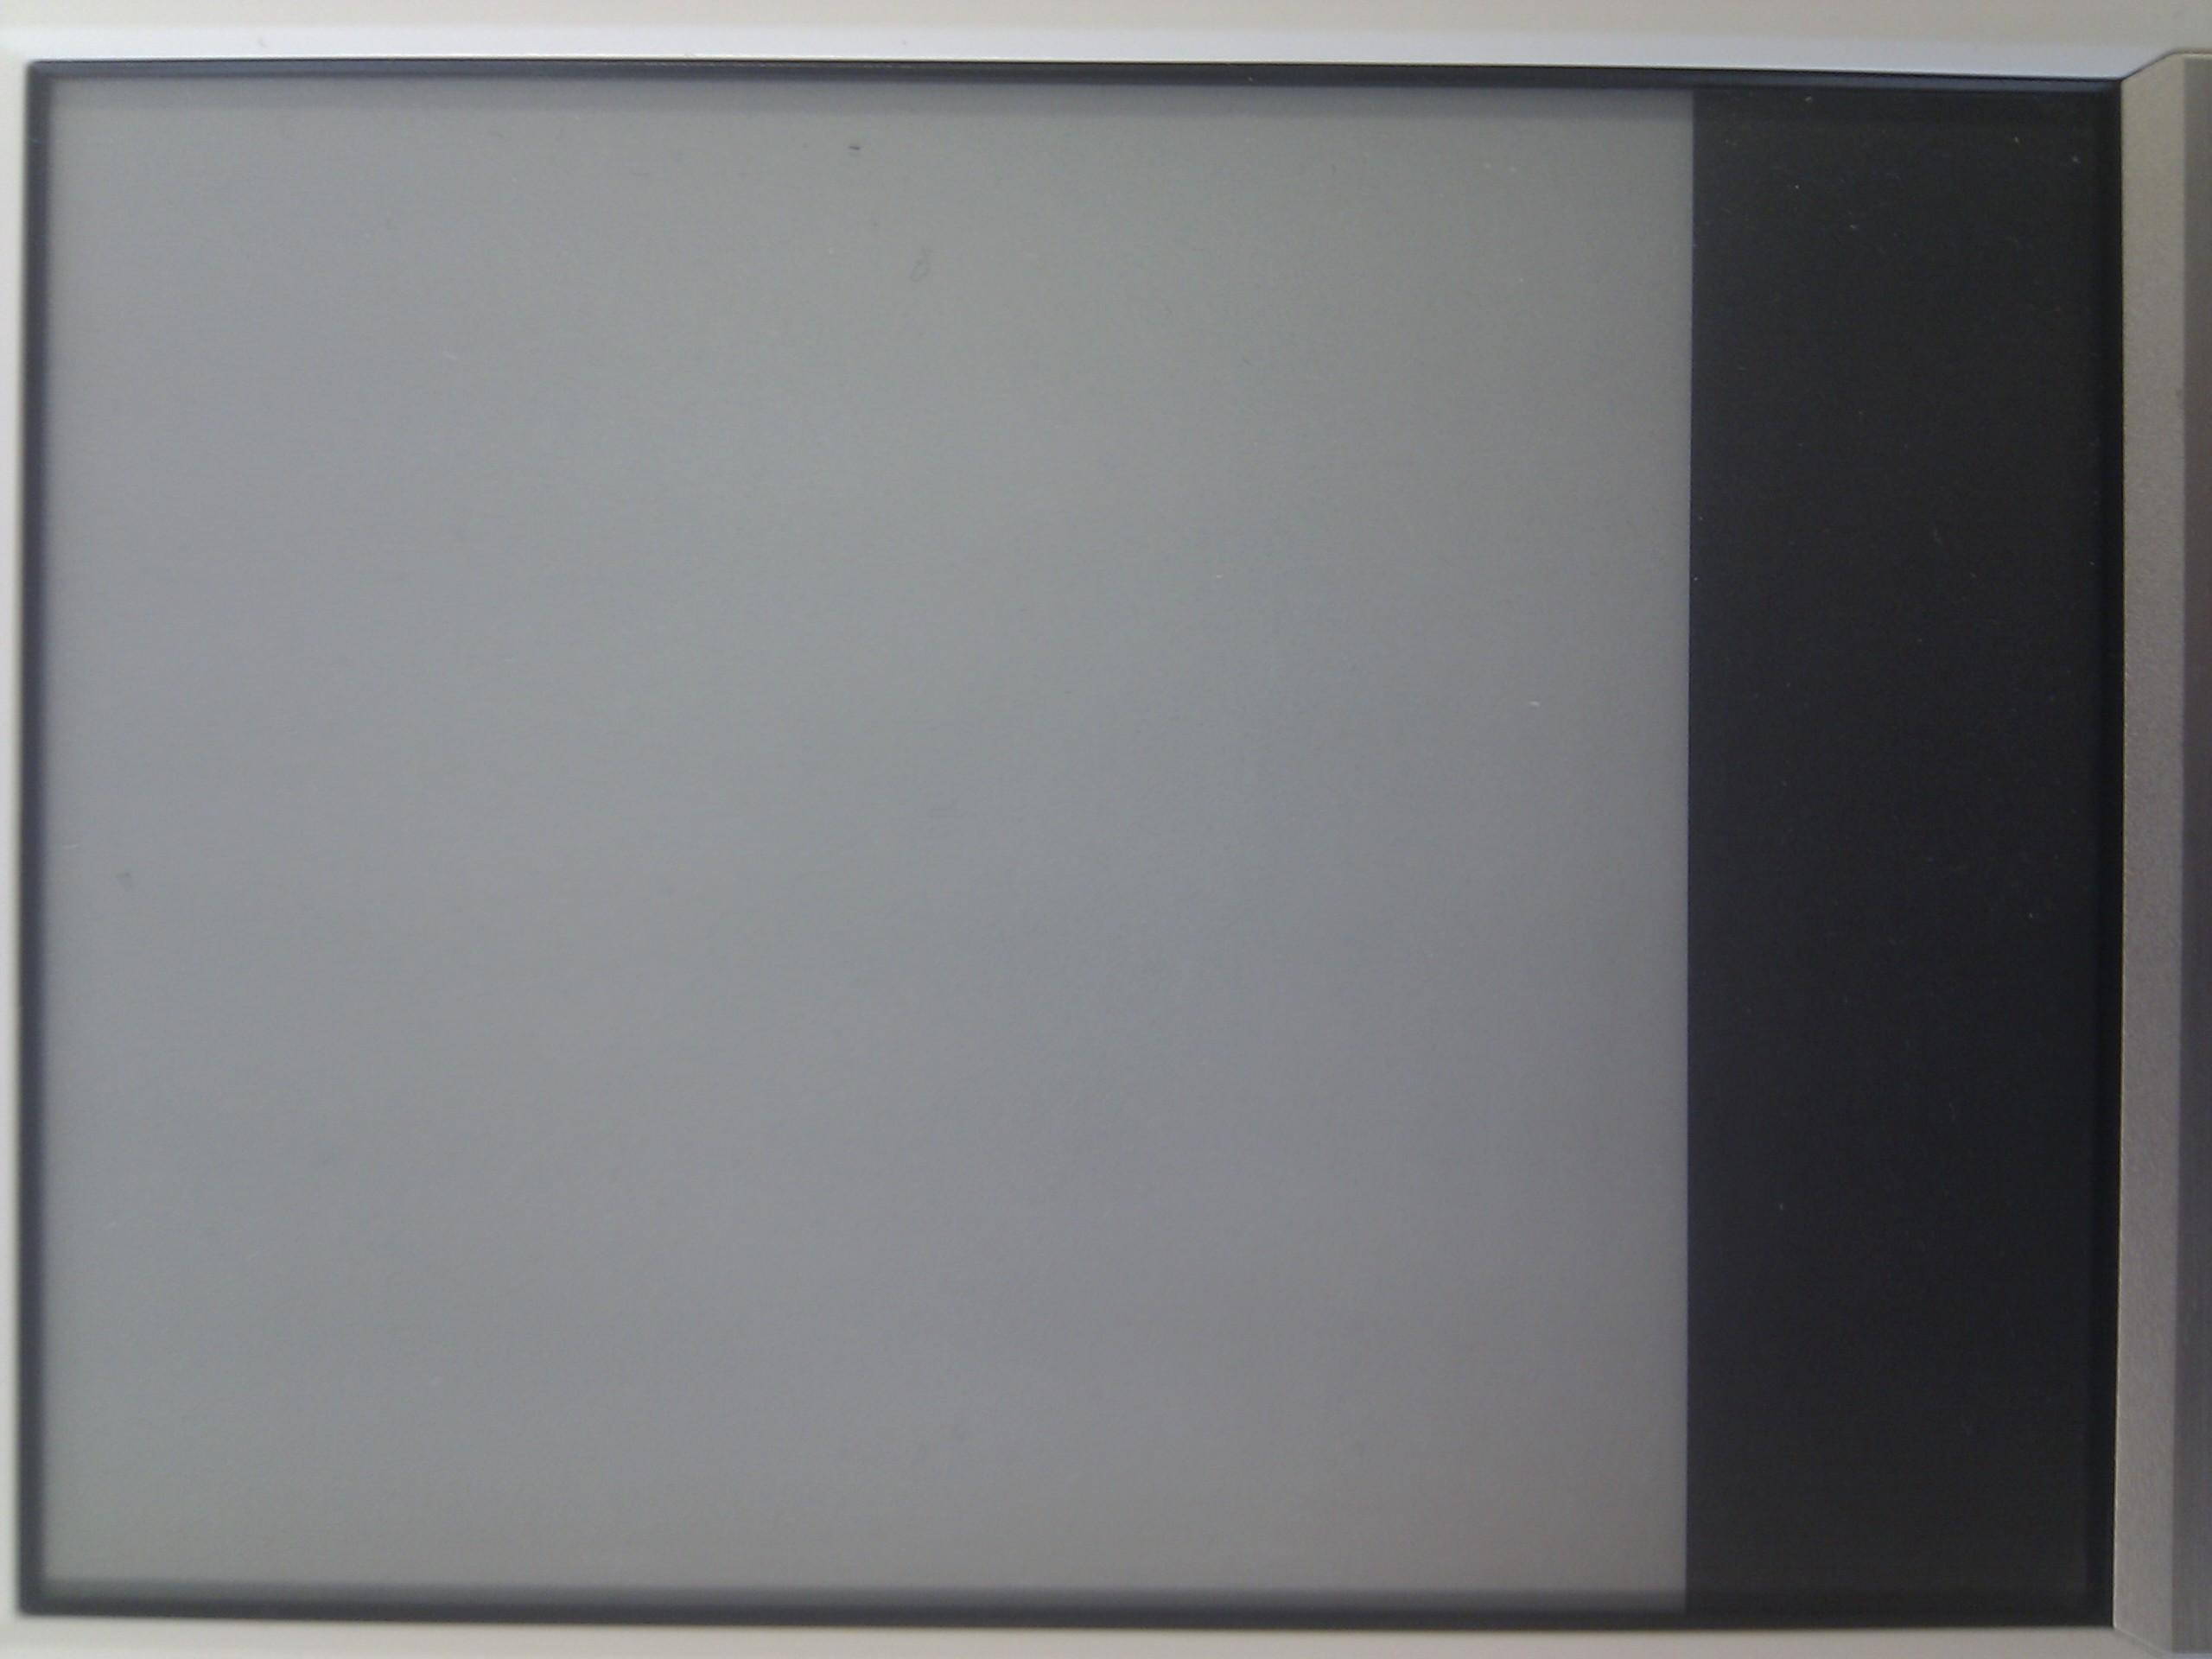
\includegraphics[angle=-90,origin=c,scale=0.04]{du_a2.jpg}
		}
		\parbox{0.6\linewidth}{
			\begin{itemize}
				\item DU ou A2
				\begin{itemize}
					\item seulement 2 niveaux de gris
					\item temps de rafraîchissement : 
					\begin{itemize}
						\item mesuré  : 126ms (A2) 280ms (DU)
						\item annoncé  : 300ms
					\end{itemize}		
				\end{itemize}
			\end{itemize}
		}
	\end{block}
\end{frame}

\begin{frame}{ Affichage via DirectFB }
	\begin{block} { Différence d'affichage entre les waveformes }
		\parbox{0.3\linewidth}{
			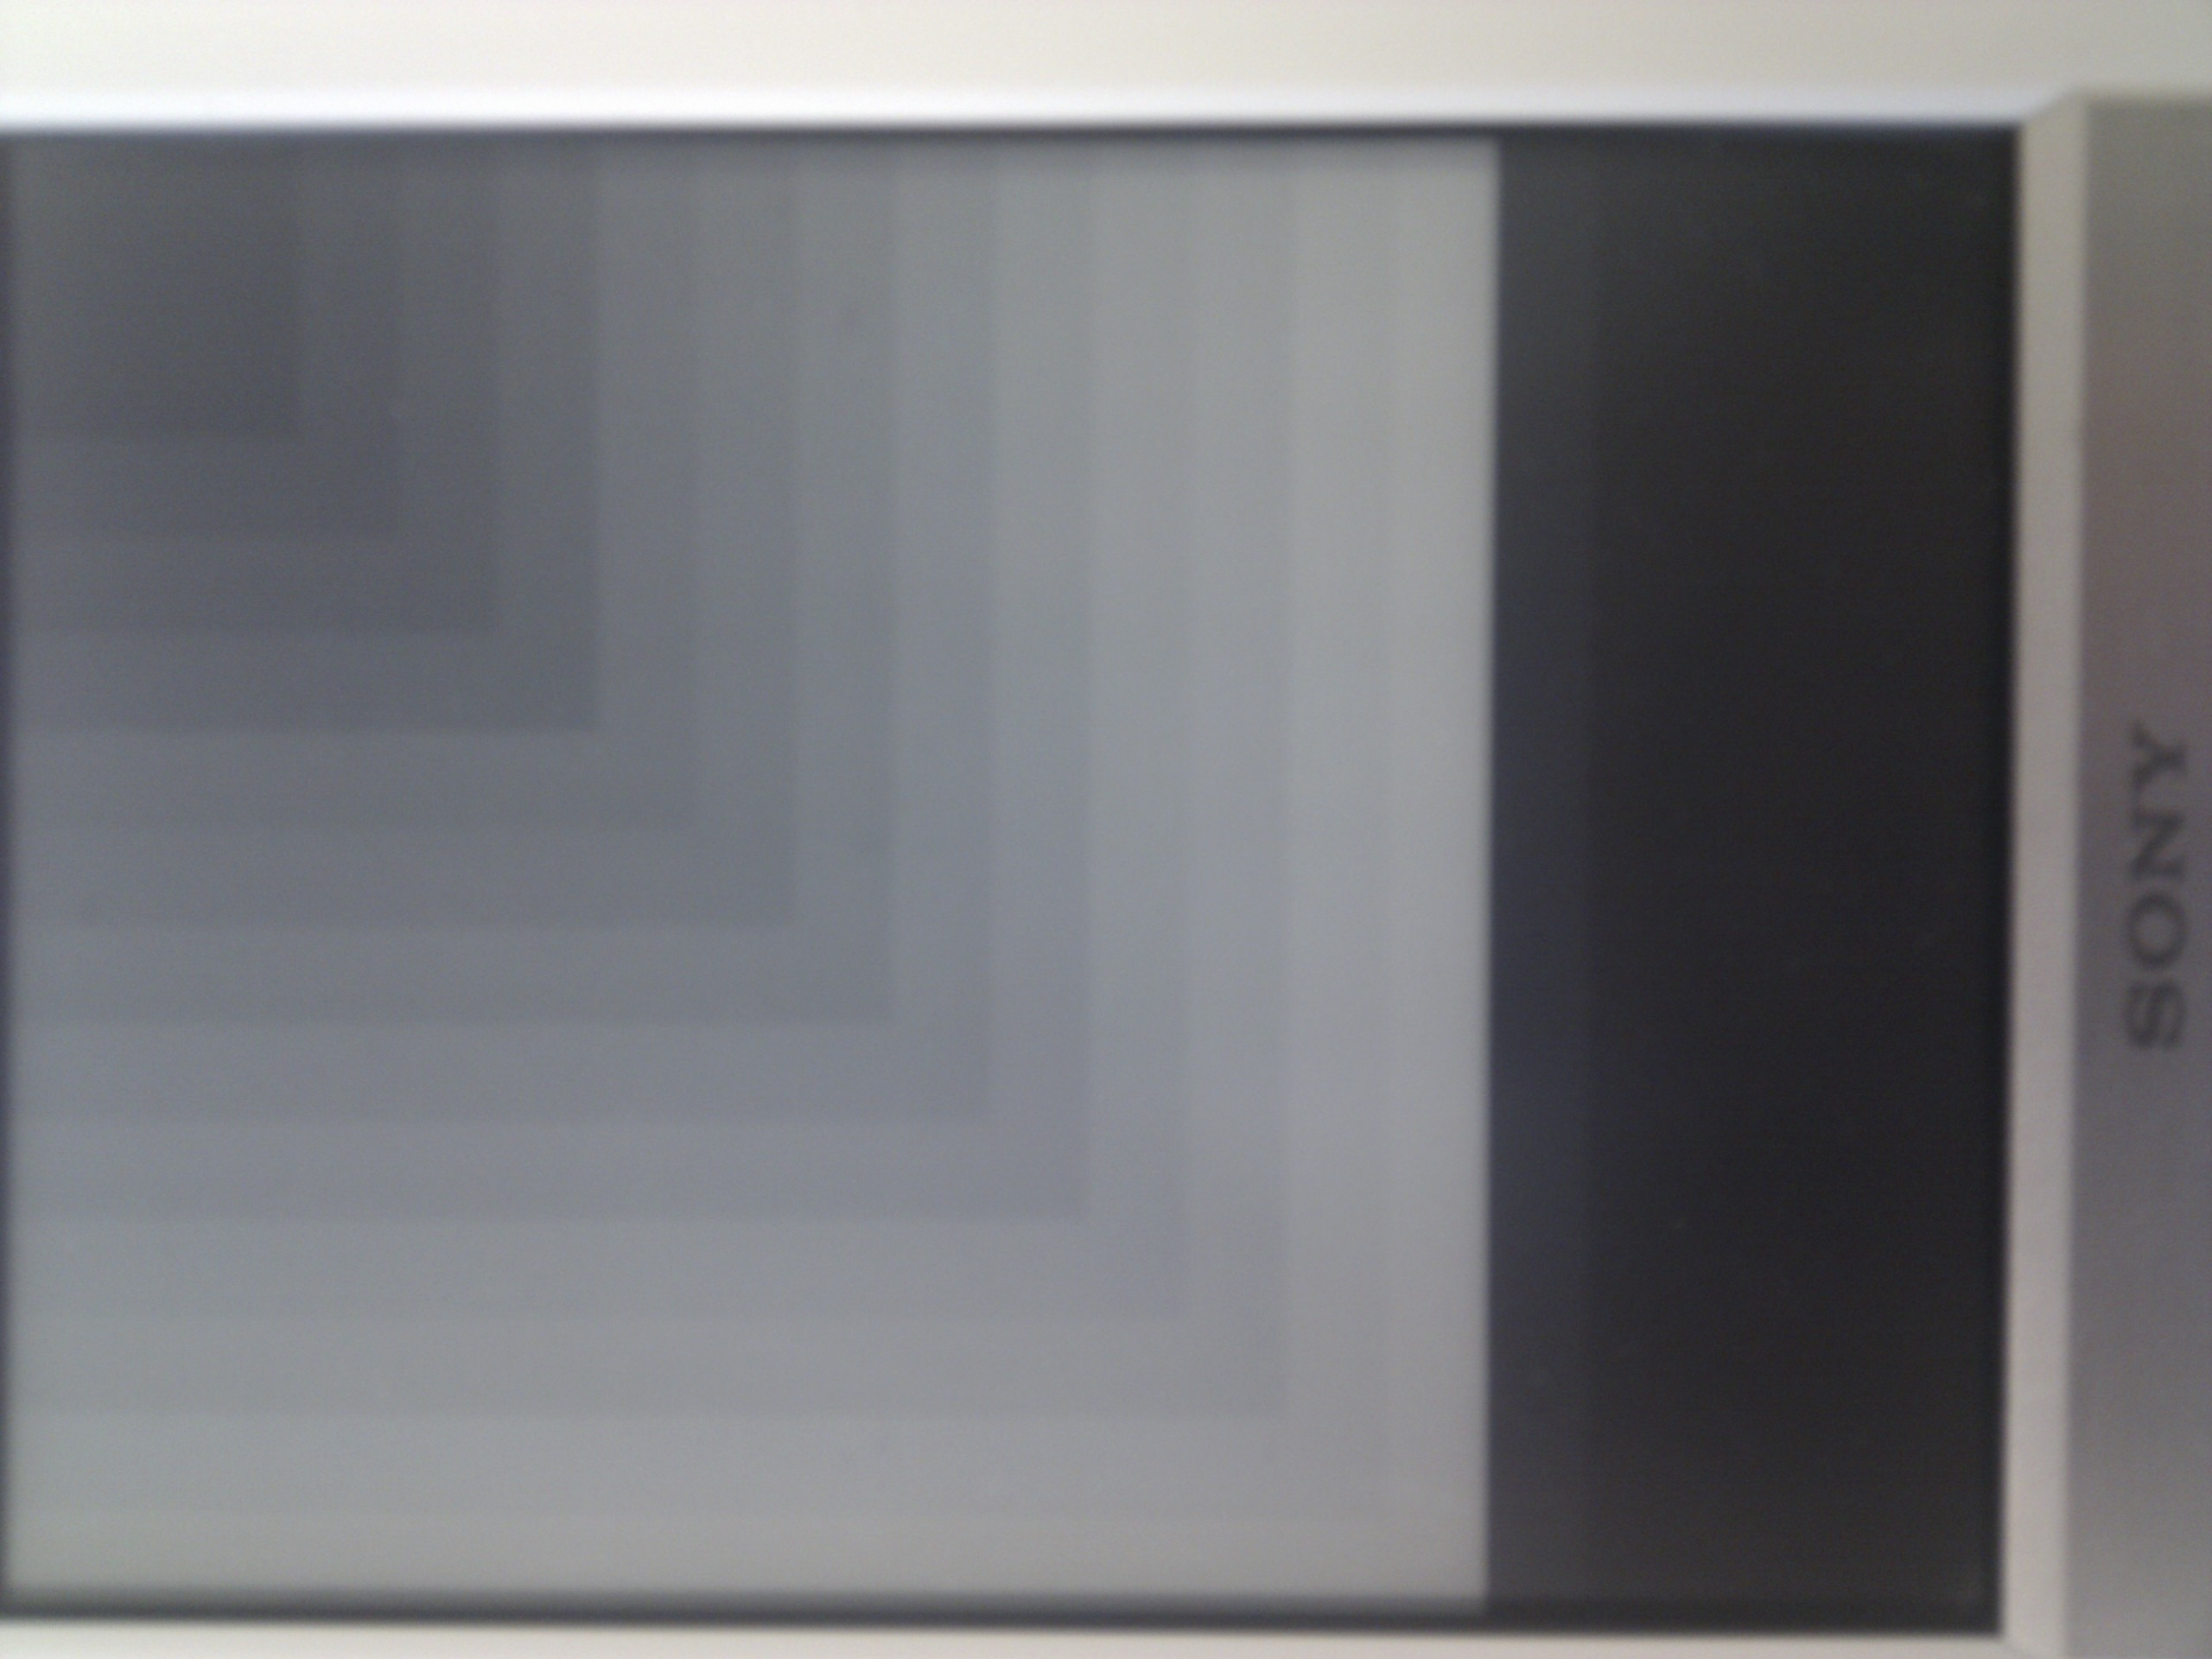
\includegraphics[angle=-90,origin=c,scale=0.04]{gc4_8.jpg}
		}
		\parbox{0.6\linewidth}{
			\begin{itemize}
				\item GC4
				\begin{itemize}
					\item 4 niveaux de gris
					\item temps de rafraîchissement : 
					\begin{itemize}
						\item mesuré  : 610ms
						\item annoncé  : 600ms
					\end{itemize}		
				\end{itemize}
			\end{itemize}
		}
	\end{block}
\end{frame}

\begin{frame}{ Affichage via DirectFB }
	\begin{block} { Différence d'affichage entre les waveformes }
		\parbox{0.3\linewidth}{
			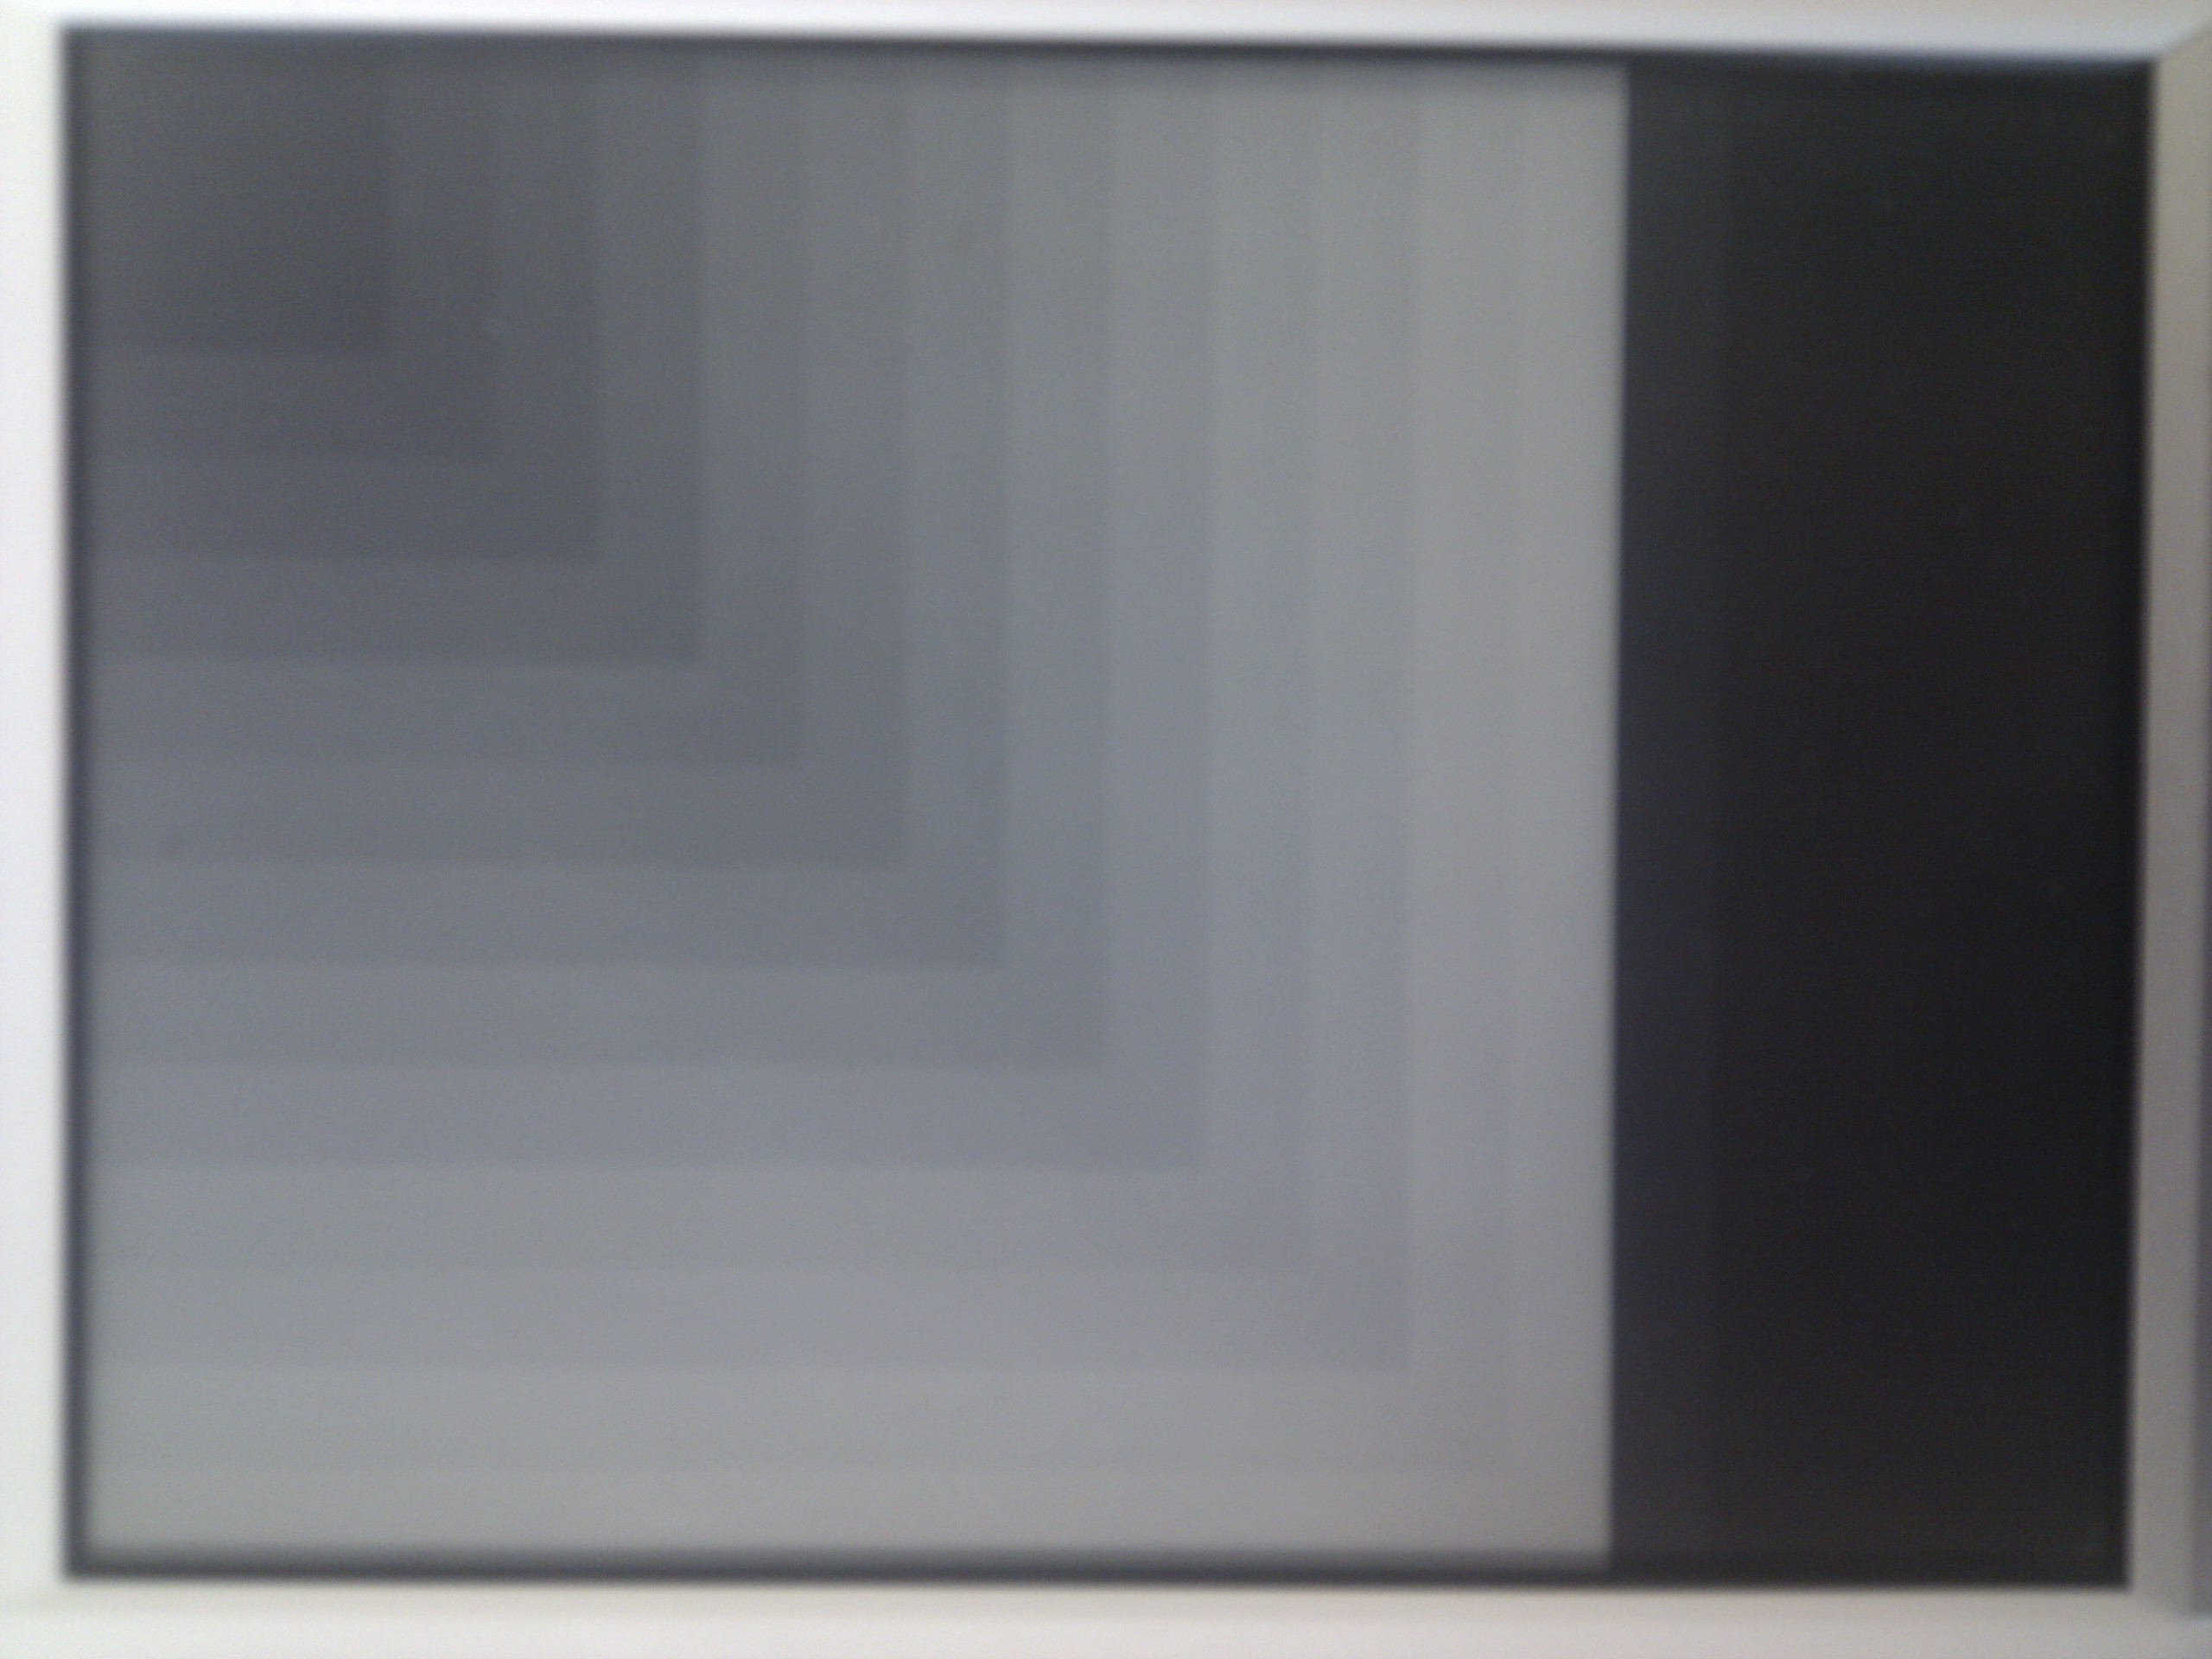
\includegraphics[angle=-90,origin=c,scale=0.04]{gc8_4.jpg}
		}
		\parbox{0.6\linewidth}{
			\begin{itemize}
				\item GC8 ou GC16
				\begin{itemize}
					\item 16 niveaux de gris
					\item temps de rafraîchissement : 
					\begin{itemize}
						\item mesuré  : 610ms
						\item annoncé  : 900ms
					\end{itemize}		
				\end{itemize}
			\end{itemize}
		}
	\end{block}
\end{frame}
\section[Bilan]{Bilan du projet}
\subsection[État actuel]{État actuel du projet}
\begin{frame}{État actuel du projet}

\begin{block}{État d'avancement}

	\begin{itemize}
		\item Connexion Ethernet entre la liseuse et un PC hôte :
		\begin{itemize}
			\item via le port USB
			\item émulation d'une connexion Ethernet
			\item utilisation possible du protocole SSH
		\end{itemize}
		\item Modification de l'affichage de l'écran
		\begin{itemize}
			\item programme utilisant DirectFB
			\item mise à jour de l'affichage via ioctl
		\end{itemize}
	\end{itemize}

\end{block}

\end{frame}

\subsection[Suite]{Suite du projet}
\begin{frame}{Suite du projet}

\begin{block}{VNC}
	\begin{itemize}
		\item Client sur le PC hôte
		\item Serveur sur la liseuse
		\item Traitements côté client
		\item Modification du protocole RFB
	\end{itemize}
\end{block}

\begin{block}{QEMU}
	\begin{itemize}
		\item Configurer QEMU pour utiliser VNC
		\item Configurer l'image pour l'utiliser avec QEMU
	\end{itemize}
\end{block}

\end{frame}


\end{document}